\documentclass[a4paper, 17pt]{extarticle}

% page margin
\usepackage[margin=2cm]{geometry}
% to use russian language
\usepackage[utf8]{inputenc}
\usepackage[russian]{babel}
% to write math
\usepackage{amsmath, amsthm, amssymb}
% to use links
\usepackage[colorlinks=true, linkcolor=red]{hyperref}
% to use "" properly
\usepackage{csquotes}
% for work with pictures
\usepackage{float}
\usepackage{wrapfig}
\usepackage[thinlines]{easytable}
\usepackage{subcaption}
\usepackage{graphicx}
\graphicspath{ {./pics/} }

\begin{document}
\begin{titlepage}
  \begin{center}
    \small{ \bfseries{
    МИНИСТЕРСТВО ЦИФРОВОГО \\ РАЗВИТИЯ, СВЯЗИ И \\ МАССОВЫХ
    КОММУНИКАЦИЙ \\ РОССИЙСКОЙ ФЕДЕРАГИИ \\ Ордена Трудового Красного
    Знамени федеральное государственное бюджетное учреждение высшего
    образования \enquote{Московский технический университет связи и
    информатики}}\\
  \mdseries}

    \vspace{1.7cm}

    \normalsize{Кафедра \enquote{Информационные технологии}} \\
    \normalsize{Предмет \enquote{Математические Основы Баз Данных}}

    \vspace{0.3cm}
    \huge{Лабораторная работа №1} \\
    \large{\textbf{Нахождение простых чисел и выявления палидрома}} \\
    \vspace{0.3cm}
    % \normalsize{\textit{Вариант}}

    \vspace{2.7cm}

    \raggedleft 
    \normalsize{Выполнил: \\ студент гр. БПИ2402 
    \\\vspace{0.125cm} Поляков Н.А.\\}
    \centering

    \vspace{\fill}

    Москва \\ 2025

  \end{center}
\end{titlepage}

\tableofcontents
\pagebreak

\section{Цель работы}
Закрепить теоретические навыки программирования на языке Java, полученные на
лекциях и в ходе самостоятельных работ. Научиться работать с циклами, методами,
строками, а также самостоятельно реализовывать простейшие алгоритмы.
\section{Индивидуальное задание}
\begin{enumerate}
  \item Создать программу, когда находит все простые числа от 2 до 100.
  \item Создать программу, которая определяет, являются ли вводимые пользователем
  строки палидромами
\end{enumerate}

\pagebreak

\section{Демонстрация}

\begin{figure}[h]
  \centering
  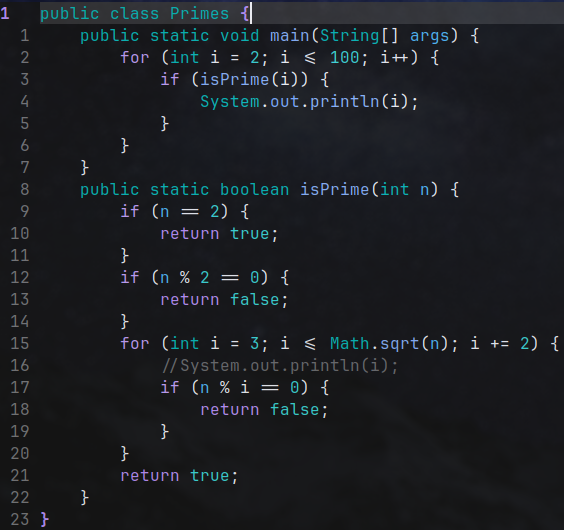
\includegraphics[width=.4\textwidth]{primes.png}
  \caption{Программа поиска простых чисел}
\end{figure}

\begin{figure}[h]
  \centering
  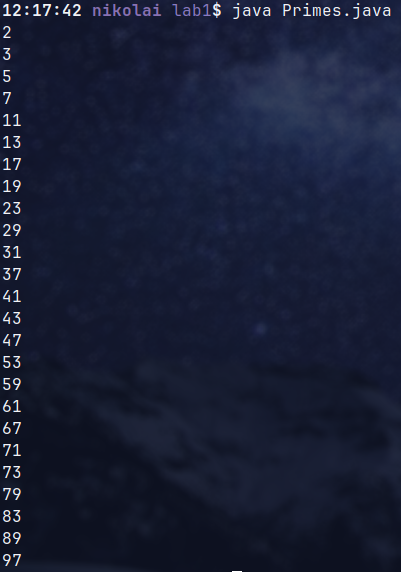
\includegraphics[width=.4\textwidth]{primes_output.png}
  \caption{}
\end{figure}

\begin{figure}[h]
  \centering
  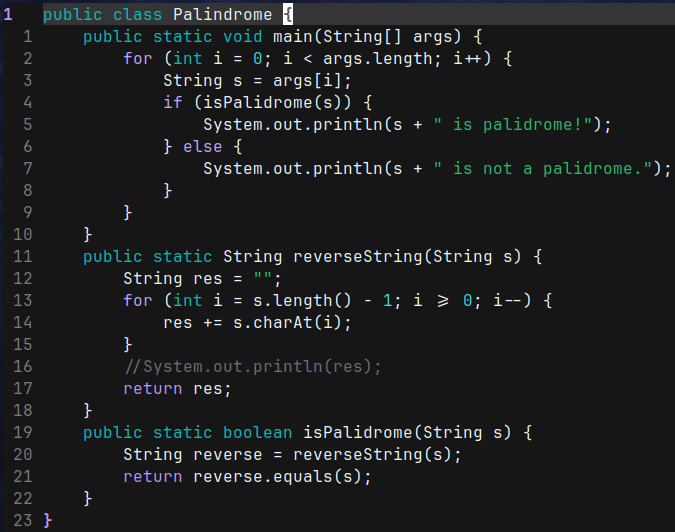
\includegraphics[width=.6\textwidth]{palidrome.png}
  \caption{Программа поиска палидромов}
\end{figure}
\begin{figure}[h]
  \centering
  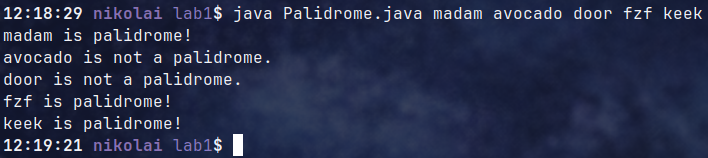
\includegraphics[width=.6\textwidth]{palidrome_output.png}
  \caption{}
\end{figure}

\pagebreak
\section{Вывод}
В ходе лабораторной работы я закрепил навыки программирования на Java, работать
с циклами, методами и строками.

\section{\href{https://github.com/KLARKOFF/IT-and-Programming-labs}{Github}}

\end{document}

